\documentclass[tikz,convert={outext=.png}]{standalone}
\begin{document}
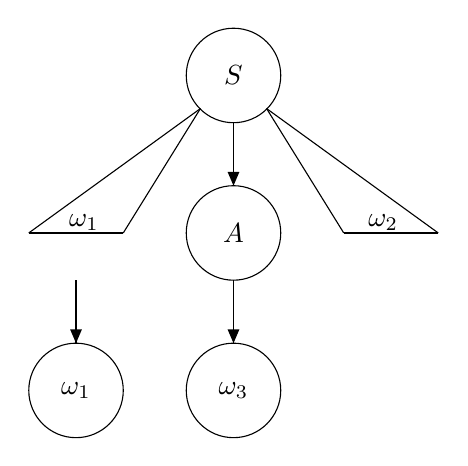
\begin{tikzpicture}[scale=0.2]
\tikzstyle{every node}+=[inner sep=0pt]
\draw [black] (0,0) circle (3);
\draw (0,0) node {$S$};

\draw [black] (-2.1, -2.1) -- (-7,-10);
\draw [black] (-2.1, -2.1) -- (-13,-10);
\draw [black, thick] (-7,-10) -- (-13, -10);
\draw (-9.5, -9.875) node [above] {$\omega_1$};

\draw [black] (0, -3) -- (0, -7);
\fill [black] (0, -7) -- (-.375, -6.125) -- (+.375, -6.125);
\draw [black] (0, -10) circle (3);
\draw (0, -10) node {$A$};

\draw [black] (+2.1, -2.1) -- (7,-10);
\draw [black] (+2.1, -2.1) -- (13,-10);
\draw [black, thick] (7,-10) -- (13, -10);
\draw (+9.5, -9.875) node [above] {$\omega_2$};

\draw [black] (-10, -13) -- (-10, -17);
\fill [black] (-10, -17) -- (-10.375, -16.125) -- (-9.625, -16.125);
\draw [black] (-10, -20) circle (3);
\draw (-10, -20) node {$\omega_1$};

\draw [black] (0, -13) -- (0, -17);
\fill [black] (0, -17) -- (-.375, -16.125) -- (+.375, -16.125);
\draw [black] (0, -20) circle (3);
\draw (0, -20) node {$\omega_3$};

\end{tikzpicture}
\end{document}
